\documentclass[11pt,a4paper]{report}
\usepackage[textwidth=37em,vmargin=30mm]{geometry}
\usepackage{calc,xunicode,amsmath,amssymb,paralist,enumitem,tabu,booktabs,datetime2,xeCJK,xeCJKfntef,listings}
\usepackage{tocloft,fancyhdr,tcolorbox,xcolor,graphicx,eso-pic,xltxtra,xelatexemoji}

\newcommand{\envyear}[0]{2024}
\newcommand{\envdatestr}[0]{2024-10-30}
\newcommand{\envfinaldir}[0]{webdb/2024/20241030/final}

\usepackage[hidelinks]{hyperref}
\hypersetup{
    colorlinks=false,
    pdfpagemode=FullScreen,
    pdftitle={Web Digest - \envdatestr}
}

\setlength{\cftbeforechapskip}{10pt}
\renewcommand{\cftchapfont}{\rmfamily\bfseries\large\raggedright}
\setlength{\cftbeforesecskip}{2pt}
\renewcommand{\cftsecfont}{\sffamily\small\raggedright}

\setdefaultleftmargin{2em}{2em}{1em}{1em}{1em}{1em}

\usepackage{xeCJK,xeCJKfntef}
\xeCJKsetup{PunctStyle=plain,RubberPunctSkip=false,CJKglue=\strut\hskip 0pt plus 0.1em minus 0.05em,CJKecglue=\strut\hskip 0.22em plus 0.2em}
\XeTeXlinebreaklocale "zh"
\XeTeXlinebreakskip = 0pt


\setmainfont{Brygada 1918}
\setromanfont{Brygada 1918}
\setsansfont{IBM Plex Sans}
\setmonofont{JetBrains Mono NL}
\setCJKmainfont{Noto Serif CJK SC}
\setCJKromanfont{Noto Serif CJK SC}
\setCJKsansfont{Noto Sans CJK SC}
\setCJKmonofont{Noto Sans CJK SC}

\setlength{\parindent}{0pt}
\setlength{\parskip}{8pt}
\linespread{1.15}

\lstset{
	basicstyle=\ttfamily\footnotesize,
	numbersep=5pt,
	backgroundcolor=\color{black!5},
	showspaces=false,
	showstringspaces=false,
	showtabs=false,
	tabsize=2,
	captionpos=b,
	breaklines=true,
	breakatwhitespace=true,
	breakautoindent=true,
	linewidth=\textwidth
}






\newcommand{\coverpic}[2]{
    % argv: itemurl, authorname
    Cover photo by #2~~(\href{#1}{#1})
}
\newcommand{\makeheader}[0]{
    \begin{titlepage}
        % \newgeometry{hmargin=15mm,tmargin=21mm,bmargin=12mm}
        \begin{center}
            
            \rmfamily\scshape
            \fontspec{BaskervilleF}
            \fontspec{Old Standard}
            \fontsize{59pt}{70pt}\selectfont
            WEB\hfill DIGEST
            
            \vfill
            % \vskip 30pt
            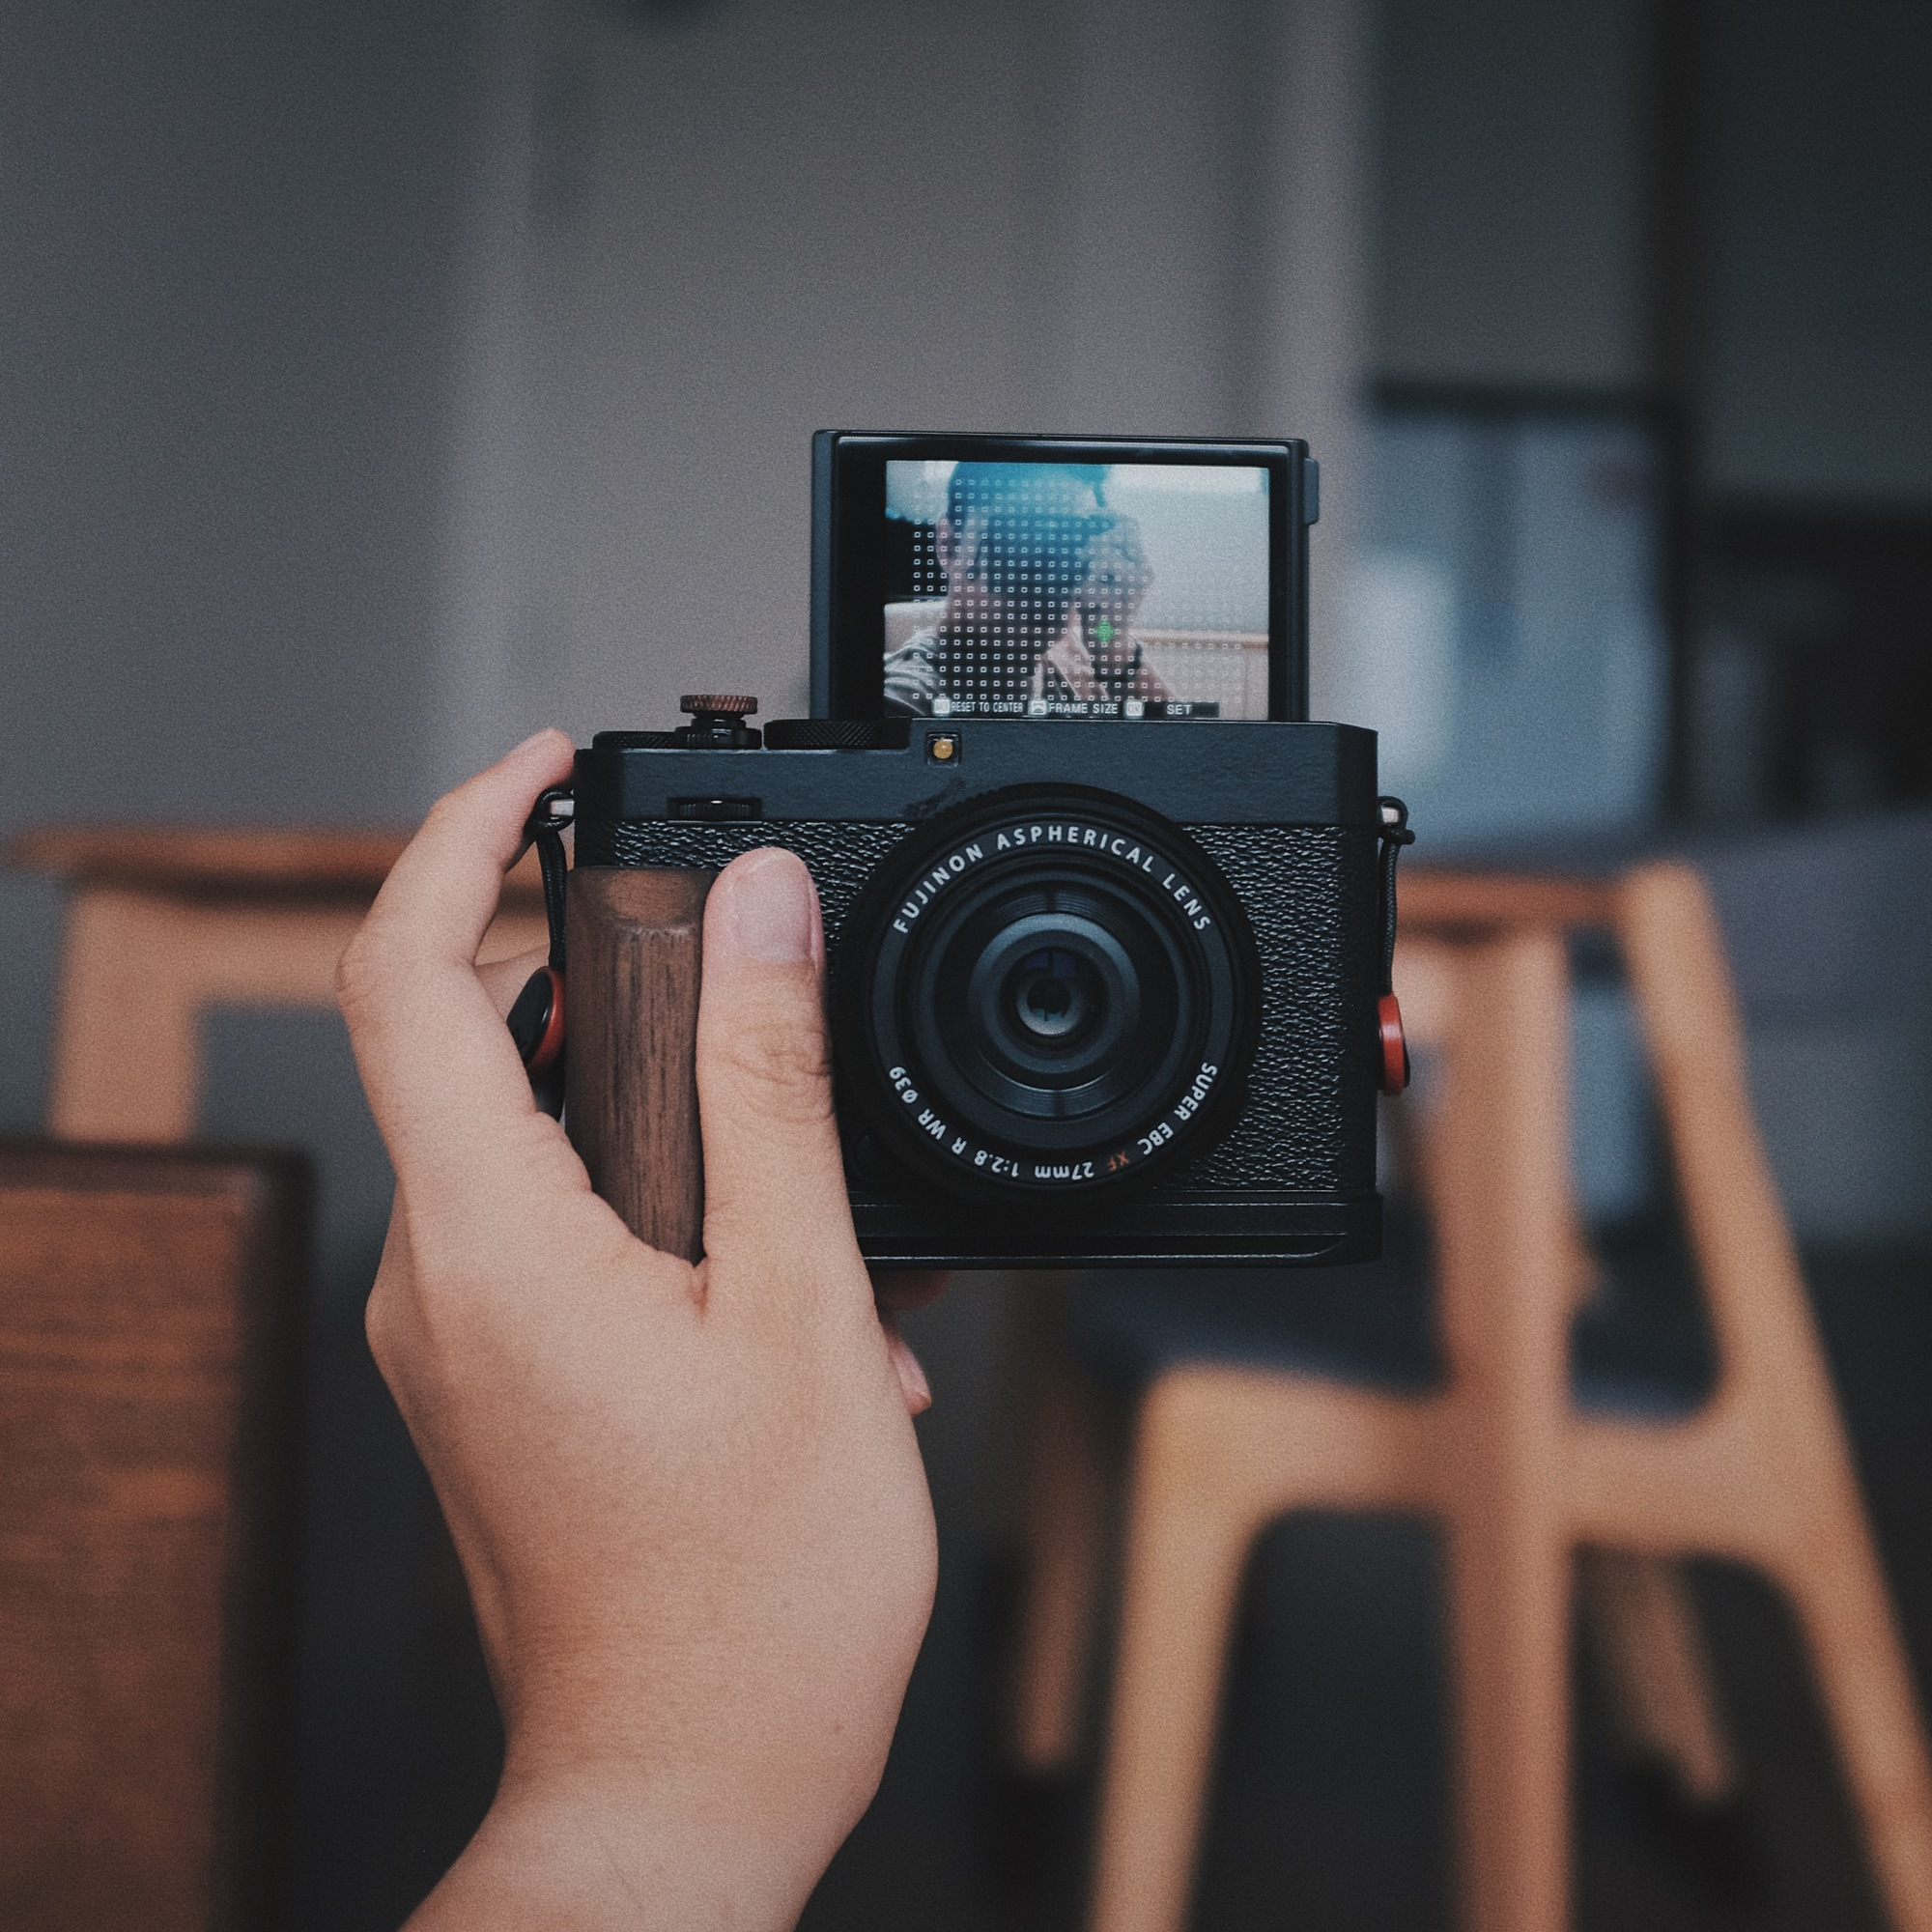
\includegraphics[width=\linewidth]{\envfinaldir/coverpic-prod.jpg}\par
            % \vskip 30pt
            \vfill

            \normalsize\rmfamily\scshape
            \copyright{} The Web Digest Project \hfill\large \envdatestr
        \end{center}
    \end{titlepage}
    % \restoregeometry
}
\newcommand{\simplehref}[1]{%
    \textcolor{blue!80!green}{\href{#1}{#1}}%
}
\renewcommand{\contentsname}{\center\Huge\sffamily\bfseries Contents\par\vskip 20pt}
\newcounter{ipartcounter}
\setcounter{ipartcounter}{0}
\newcommand{\ipart}[1]{
    % \vskip 20pt
    \clearpage
    \stepcounter{ipartcounter}
    \phantomsection
    \addcontentsline{toc}{chapter}{#1}
    % \begin{center}
    %     \Huge
    %     \sffamily\bfseries
    %     #1
    % \end{center}
    % \vskip 20pt plus 7pt
}
\newcounter{ichaptercounter}
\setcounter{ichaptercounter}{0}
\newcommand{\ichapter}[1]{
    % \vskip 20pt
    \clearpage
    \stepcounter{ichaptercounter}
    \phantomsection
    \addcontentsline{toc}{section}{\numberline{\arabic{ichaptercounter}}#1}
    \begin{center}
        \Huge
        \sffamily\bfseries
        #1
    \end{center}
    \vskip 20pt plus 7pt
}
\newcommand{\entrytitlefont}[1]{\subsection*{\raggedright\Large\sffamily\bfseries#1}}
\newcommand{\entryitemGeneric}[2]{
    % argv: title, url
    \parbox{\linewidth}{
        \entrytitlefont{#1}\par\vskip 5pt
        \footnotesize\ttfamily\mdseries
        \simplehref{#2}
    }\vskip 11pt plus 11pt minus 1pt
}
\newcommand{\entryitemGithub}[3]{
    % argv: title, url, desc
    \parbox{\linewidth}{
        \entrytitlefont{#1}\par\vskip 5pt
        \footnotesize\ttfamily\mdseries
        \simplehref{#2}\par\vskip 5pt
        \small\rmfamily\mdseries#3
    }\vskip 11pt plus 11pt minus 1pt
}
\newcommand{\entryitemAp}[3]{
    % argv: title, url, desc
    \parbox{\linewidth}{
        \entrytitlefont{#1}\par\vskip 5pt
        \footnotesize\ttfamily\mdseries
        \simplehref{#2}\par\vskip 5pt
        \small\rmfamily\mdseries#3
    }\vskip 11pt plus 11pt minus 1pt
}
\newcommand{\entryitemHackernews}[3]{
    % argv: title, hnurl, rawurl
    % \parbox{\linewidth}{
    %     \entrytitlefont{#1}\par\vskip 5pt
    %     \footnotesize\ttfamily\mdseries
    %     \simplehref{#3}\par
    %     \textcolor{black!50}{\href{#2}{#2}}
    % }\vskip 11pt plus 11pt minus 1pt
    \begin{minipage}{\linewidth}
            \entrytitlefont{#1}\par\vskip 5pt
            \footnotesize\ttfamily\mdseries
            \simplehref{#3}\par
            \textcolor{black!50}{\href{#2}{#2}}
    \end{minipage}\par\vskip 11pt plus 11pt minus 1pt
}







\begin{document}

\makeheader

\tableofcontents\clearpage




\ipart{Developers}
\ichapter{Hacker News}
\entryitemTwoLinks{GLP-1 for Everything}{https://news.ycombinator.com/item?id=41988285}{https://www.science.org/content/blog-post/glp-1-everything}

\entryitemTwoLinks{PhD student finds lost city in Mexico jungle}{https://news.ycombinator.com/item?id=41988171}{https://www.bbc.com/news/articles/crmznzkly3go}

\entryitemTwoLinks{OpenAI builds first chip with Broadcom and TSMC, scales back foundry ambition}{https://news.ycombinator.com/item?id=41986926}{https://www.reuters.com/technology/artificial-intelligence/openai-builds-first-chip-with-broadcom-tsmc-scales-back-foundry-ambition-2024-10-29/}

\entryitemTwoLinks{Using an 8K TV as a Monitor}{https://news.ycombinator.com/item?id=41986048}{https://daniel.lawrence.lu/blog/y2023m12d15/}

\entryitemTwoLinks{GitHub cuts AI deals with Google, Anthropic}{https://news.ycombinator.com/item?id=41985915}{https://www.bloomberg.com/news/articles/2024-10-29/microsoft-s-github-unit-cuts-ai-deals-with-google-anthropic}

\entryitemTwoLinks{Vector databases are the wrong abstraction}{https://news.ycombinator.com/item?id=41985176}{https://www.timescale.com/blog/vector-databases-are-the-wrong-abstraction/}

\entryitemTwoLinks{New Mac Mini with M4}{https://news.ycombinator.com/item?id=41984519}{https://www.apple.com/newsroom/2024/10/apples-new-mac-mini-is-more-mighty-more-mini-and-built-for-apple-intelligence/}

\entryitemTwoLinks{Writing in Pictures: Richard Scarry and the art of children's literature}{https://news.ycombinator.com/item?id=41983622}{https://yalereview.org/article/chris-ware-richard-scarry}

\entryitemTwoLinks{Shopify Is Winning Salesforce Clients, Stoking E-Commerce Rivalry}{https://news.ycombinator.com/item?id=41983607}{https://www.bloomberg.com/news/articles/2024-10-29/shopify-is-winning-salesforce-clients-stoking-e-commerce-rivalry}

\entryitemTwoLinks{A deep history of Halloween}{https://news.ycombinator.com/item?id=41983412}{https://resobscura.substack.com/p/a-very-deep-history-of-halloween}

\entryitemTwoLinks{Launch HN: Integuru (YC W24) – Reverse-engineer internal APIs using LLMs}{https://news.ycombinator.com/item?id=41983409}{https://github.com/Integuru-AI/Integuru}

\entryitemTwoLinks{How to get the whole planet to send abuse complaints to your best friends}{https://news.ycombinator.com/item?id=41982698}{https://delroth.net/posts/spoofed-mass-scan-abuse/}

\entryitemTwoLinks{Insiders Stealing Instagram Usernames?}{https://news.ycombinator.com/item?id=41981289}{https://javier.computer/instagram}

\entryitemTwoLinks{What happens when people with acute psychosis meet the voices in their heads?}{https://news.ycombinator.com/item?id=41980986}{https://www.theguardian.com/news/2024/oct/29/acute-psychosis-inner-voices-avatar-therapy-psychiatry}

\entryitemTwoLinks{Show HN: I built an app to use a QR code as my doorbell}{https://news.ycombinator.com/item?id=41980681}{https://dingdongdoorbell.com}

\entryitemTwoLinks{How I write code using Cursor}{https://news.ycombinator.com/item?id=41979203}{https://www.arguingwithalgorithms.com/posts/cursor-review.html}

\entryitemTwoLinks{The electrostatic world of insects}{https://news.ycombinator.com/item?id=41978478}{https://www.wired.com/story/the-secret-electrostatic-world-of-insects/}

\entryitemTwoLinks{An indie studio created a game based on Stanislaw Lem's novel}{https://news.ycombinator.com/item?id=41978246}{https://invinciblethegame.com/?hn}

\entryitemTwoLinks{What's New in POSIX 2024}{https://news.ycombinator.com/item?id=41978197}{https://blog.toast.cafe/posix2024-xcu}

\entryitemTwoLinks{Why Slight Failed: A Slight Post-Mortem}{https://news.ycombinator.com/item?id=41977205}{https://www.colmanhumphrey.com/posts/why-slight-failed/}\ichapter{Phoronix}
\entryitemGeneric{\hskip 0pt{}Coreboot Issues Rebuttal To Recent Laptop Vendor Controversy}{https://www.phoronix.com/news/Coreboot-Rebuttal-MALIBAL}

\entryitemGeneric{\hskip 0pt{}Linux Use On Microsoft Azure Crosses 60\%, AlmaLinux Now An Endorsed Distro}{https://www.phoronix.com/news/Azure-Endorses-AlmaLinux}

\entryitemGeneric{\hskip 0pt{}Local Privilege Escalation Vulnerability Affecting X.Org Server For 18 Years}{https://www.phoronix.com/news/X.Org-CVE-2024-9632}

\entryitemGeneric{\hskip 0pt{}Crucial Pro DDR5-6400 32GB Kit Performance With Intel Arrow Lake}{https://www.phoronix.com/review/crucial-pro-ddr5-6400}

\entryitemGeneric{\hskip 0pt{}Fedora 41 Releases Today With Many Shiny New Features}{https://www.phoronix.com/news/Fedora-41-Download}

\entryitemGeneric{\hskip 0pt{}RISC-V User-Space Pointer Masking Appears Ready For Linux 6.13}{https://www.phoronix.com/news/RISC-V-Pointer-Masking-Linux}

\entryitemGeneric{\hskip 0pt{}Linux Patches Aim To Further Lower Intel Sierra Forest Idle Power Use}{https://www.phoronix.com/news/Xeon-6-SRF-Idle-Lower-Deeper}

\entryitemGeneric{\hskip 0pt{}RADV Vulkan Driver Merges Device Generated Commands Support}{https://www.phoronix.com/news/RADV-VK-EXT-DGC}

\entryitemGeneric{\hskip 0pt{}Google's Flutter UI Toolkit Forked As Flock}{https://www.phoronix.com/news/Google-Flutter-UI-Flock-Fork}


\ipart{Developers~~~~(zh-Hans)}
\ichapter{Solidot}
\entryitemGeneric{\hskip 0pt{}Meta 开发 AI 搜索引擎}{https://www.solidot.org/story?sid=79625}

\entryitemGeneric{\hskip 0pt{}俄罗斯从马来西亚借道印度购买英伟达芯片}{https://www.solidot.org/story?sid=79624}

\entryitemGeneric{\hskip 0pt{}美国从明年 1 月起限制半导体和 AI 领域的对华投资}{https://www.solidot.org/story?sid=79623}

\entryitemGeneric{\hskip 0pt{}X 认证用户助长极化}{https://www.solidot.org/story?sid=79622}

\entryitemGeneric{\hskip 0pt{}苹果将教育游戏《俄勒冈小径》改编为电影}{https://www.solidot.org/story?sid=79621}

\entryitemGeneric{\hskip 0pt{}随着年龄增长鸟儿的朋友也会越来越少}{https://www.solidot.org/story?sid=79620}

\entryitemGeneric{\hskip 0pt{}Linus Torvalds 认为 AI 九成是营销一成才是现实}{https://www.solidot.org/story?sid=79619}

\entryitemGeneric{\hskip 0pt{}使用 AI 创建儿童色情的英国男子被判 18 年}{https://www.solidot.org/story?sid=79618}

\entryitemGeneric{\hskip 0pt{}联邦宇宙平台有了自己的短视频应用 Loops}{https://www.solidot.org/story?sid=79617}

\entryitemGeneric{\hskip 0pt{}在贝佐斯拒绝华盛顿邮报为贺锦丽背书之后愈 20 万订户取消订阅}{https://www.solidot.org/story?sid=79616}

\entryitemGeneric{\hskip 0pt{}Google Chrome 将引入 AI 执行填写表格、购物和定航班功能}{https://www.solidot.org/story?sid=79615}

\entryitemGeneric{\hskip 0pt{}美国版权局拒绝用于游戏保存的 DMCA 豁免}{https://www.solidot.org/story?sid=79614}

\entryitemGeneric{\hskip 0pt{}《终结者》对 AI 的刻画仍然影响我们在 AI 上的立场}{https://www.solidot.org/story?sid=79613}

\entryitemGeneric{\hskip 0pt{}V404 黑洞双星系统被发现是三天体系统}{https://www.solidot.org/story?sid=79612}

\entryitemGeneric{\hskip 0pt{}Instagram 和 Meta 会降低低观看量视频的质量 }{https://www.solidot.org/story?sid=79610}

\entryitemGeneric{\hskip 0pt{}开源本身不是科技巨头服务的替代}{https://www.solidot.org/story?sid=79609}

\entryitemGeneric{\hskip 0pt{}韦伯望远镜发现了流浪类星体}{https://www.solidot.org/story?sid=79608}

\entryitemGeneric{\hskip 0pt{}昆虫因人为环境变化而改变颜色}{https://www.solidot.org/story?sid=79607}

\entryitemGeneric{\hskip 0pt{}Gentoo 引入了 DTrace}{https://www.solidot.org/story?sid=79606}

\entryitemGeneric{\hskip 0pt{}欧洲犯罪组织天天炸 ATM}{https://www.solidot.org/story?sid=79605}\ichapter{V2EX}
\entryitemGeneric{\hskip 0pt{}[Apple] 心心念的 mac mini 一线通还是实现不了啊}{https://www.v2ex.com/t/1084797}

\entryitemGeneric{\hskip 0pt{}[Apple] 家里有 NAS 的话怎么选 Mac mini?}{https://www.v2ex.com/t/1084795}

\entryitemGeneric{\hskip 0pt{}[问与答] 大佬们 5000 预算是游戏笔记本,还是主机+显示器?}{https://www.v2ex.com/t/1084794}

\entryitemGeneric{\hskip 0pt{}[问与答] 想买两块屏幕写代码用}{https://www.v2ex.com/t/1084793}

\entryitemGeneric{\hskip 0pt{}[iPhone] iOS 18.1 通话录音的转写}{https://www.v2ex.com/t/1084792}

\entryitemGeneric{\hskip 0pt{}[GitHub Copilot] GitHub Copilot for Xcode}{https://www.v2ex.com/t/1084791}

\entryitemGeneric{\hskip 0pt{}[宽带症候群] 关于 Arm 软路由使用体验不如 X86 软路由}{https://www.v2ex.com/t/1084790}

\entryitemGeneric{\hskip 0pt{}[Apple] 国行 Mac 和 Apple Intelligence 之间有生殖隔离吗}{https://www.v2ex.com/t/1084789}

\entryitemGeneric{\hskip 0pt{}[推广] 和 Ai 磕了三个小时,也做出了人生中的第 1 个 [独立开发] Web APP🥳}{https://www.v2ex.com/t/1084788}

\entryitemGeneric{\hskip 0pt{}[Apple] mac mini m4 配置怎么选?}{https://www.v2ex.com/t/1084787}

\entryitemGeneric{\hskip 0pt{}[iPad] 手里的 iPad air2 太老了,求更换建议。}{https://www.v2ex.com/t/1084786}

\entryitemGeneric{\hskip 0pt{}[YouTube] 求推荐油管频道,适合吃饭时候作为电子榨菜的}{https://www.v2ex.com/t/1084785}

\entryitemGeneric{\hskip 0pt{}[软件] Windows 端有什么好用的远程控制软件吗?}{https://www.v2ex.com/t/1084784}

\entryitemGeneric{\hskip 0pt{}[分享创造] SAT Score Calculator: Your Ultimate SAT Prep Tool}{https://www.v2ex.com/t/1084783}

\entryitemGeneric{\hskip 0pt{}[分享创造] 新上线小游戏: Sprunki, https://sprunki.im/}{https://www.v2ex.com/t/1084780}

\entryitemGeneric{\hskip 0pt{}[iCloud] mac 上 Safari 首没有 iCloud 标签选项了}{https://www.v2ex.com/t/1084779}

\entryitemGeneric{\hskip 0pt{}[Apple] M4 基础款支持三显示器了}{https://www.v2ex.com/t/1084777}

\entryitemGeneric{\hskip 0pt{}[分享发现] 分享一本新发现的很好看的科幻(异能)小说《战略级天使》}{https://www.v2ex.com/t/1084776}

\entryitemGeneric{\hskip 0pt{}[MacBook Pro] M4pro 的 Mac mini 上雷电 5 了,明晚发布的 M4pro/max 的 MBP 也会有雷电 5 吗}{https://www.v2ex.com/t/1084775}

\entryitemGeneric{\hskip 0pt{}[分享创造] 经过几个月的开发, eno-m 非常好用了已经🥵}{https://www.v2ex.com/t/1084774}

\entryitemGeneric{\hskip 0pt{}[Apple] 我要冲 Mac mini m4,不过要等 20 来天估计,旧款 M2 得先卖掉,希望不要亏太多}{https://www.v2ex.com/t/1084773}

\entryitemGeneric{\hskip 0pt{}[程序员] 新 M4 Mac Mini 出了,起步 16 G - 3749,值不值得买?}{https://www.v2ex.com/t/1084772}

\entryitemGeneric{\hskip 0pt{}[Apple] Mac mini m4 发布了}{https://www.v2ex.com/t/1084771}

\entryitemGeneric{\hskip 0pt{}[Apple] 新款	Mac mini 如何开关机?}{https://www.v2ex.com/t/1084770}

\entryitemGeneric{\hskip 0pt{}[问与答] 求推荐一个看剧的大屏安卓平板}{https://www.v2ex.com/t/1084769}

\entryitemGeneric{\hskip 0pt{}[Apple] Mac mini M4 怎样选}{https://www.v2ex.com/t/1084768}

\entryitemGeneric{\hskip 0pt{}[微信] 微信小程序走代理, dns 泄漏,求解决办法}{https://www.v2ex.com/t/1084767}

\entryitemGeneric{\hskip 0pt{}[Apple] Mac Mini M4 Pro 带雷点 5 接口}{https://www.v2ex.com/t/1084766}

\entryitemGeneric{\hskip 0pt{}[Apple] Mac mini 已经发布了,明天晚上 11 点发布 Macbook Pro}{https://www.v2ex.com/t/1084765}

\entryitemGeneric{\hskip 0pt{}[Apple] 2024 款 Mac Mini 已经发布}{https://www.v2ex.com/t/1084764}

\entryitemGeneric{\hskip 0pt{}[分享发现] 这个社区真有意思,别人骂你,但你不能骂对方,不然就会被禁回复 480 天。[笑哭]}{https://www.v2ex.com/t/1084762}

\entryitemGeneric{\hskip 0pt{}[酷工作] 想入门下 web3 项目,有偿寻求 web3 钱包开发老师}{https://www.v2ex.com/t/1084761}

\entryitemGeneric{\hskip 0pt{}[宽带症候群] 超过 10 终端 的企业用户 就应该安装 5g 599 套餐起步}{https://www.v2ex.com/t/1084760}

\entryitemGeneric{\hskip 0pt{}[分享发现] 发现 edge 浏览器积分兑换的东西又变多了啊}{https://www.v2ex.com/t/1084759}

\entryitemGeneric{\hskip 0pt{}[宽带症候群] 欧洲赛博回国求教}{https://www.v2ex.com/t/1084758}

\entryitemGeneric{\hskip 0pt{}[Cloudflare] 对象云存储+Cloudflare 可以免流量分发:这个是默认的吗,还是要单独设置?}{https://www.v2ex.com/t/1084756}

\entryitemGeneric{\hskip 0pt{}[分享发现] 推荐两千左右拍照手机}{https://www.v2ex.com/t/1084755}

\entryitemGeneric{\hskip 0pt{}[投资] 普通老百姓能买到的消息股,独角兽+高护城河}{https://www.v2ex.com/t/1084754}

\entryitemGeneric{\hskip 0pt{}[NAS] TS464C2 买入总结以及使用建议}{https://www.v2ex.com/t/1084753}

\entryitemGeneric{\hskip 0pt{}[Android] 14T Pro 有问}{https://www.v2ex.com/t/1084752}

\entryitemGeneric{\hskip 0pt{}[酷工作] Follow is looking for Growth Marketing Specialists and Operation Specialists}{https://www.v2ex.com/t/1084750}

\entryitemGeneric{\hskip 0pt{}[旅行] 特种兵的西欧南欧🇪🇺两周游(10.4-10.7 法国巴黎)}{https://www.v2ex.com/t/1084749}

\entryitemGeneric{\hskip 0pt{}[程序员] MacOS 下 Chrome 自动短信填充}{https://www.v2ex.com/t/1084748}

\entryitemGeneric{\hskip 0pt{}[问与答] macOS 15 按 Cmd+Q 快捷键退出经常无效}{https://www.v2ex.com/t/1084747}

\entryitemGeneric{\hskip 0pt{}[NAS] 求大佬给个馒头,谢谢谢谢}{https://www.v2ex.com/t/1084745}

\entryitemGeneric{\hskip 0pt{}[Telegram] 今天用错了 bot API 了}{https://www.v2ex.com/t/1084744}

\entryitemGeneric{\hskip 0pt{}[游戏] 打算在抖音直播打游戏了}{https://www.v2ex.com/t/1084743}

\entryitemGeneric{\hskip 0pt{}[程序员] 继上次诉苦之后,感觉自己心态有了一点点成长(有但不多.jpg)}{https://www.v2ex.com/t/1084742}

\entryitemGeneric{\hskip 0pt{}[分享发现] 广电卡,我好像踩坑了...}{https://www.v2ex.com/t/1084741}

\entryitemGeneric{\hskip 0pt{}[NAS] 写了一个小脚本,按照 tr 中每个种子维度展示辅种站点和数量}{https://www.v2ex.com/t/1084740}


\ipart{Generic News}
\ichapter{AP News}
\entryitemWithDescription{\hskip 0pt{}Teri Garr, the offbeat comic actor of `Young Frankenstein' and `Tootsie,' has died}{https://apnews.com/article/be39482a60724c5bb81bbd8f34dfaf2d}{}

\entryitemWithDescription{\hskip 0pt{}In a first since 1938, Des Moines, Iowa, kids will trick-or-treat on Halloween}{https://apnews.com/article/26710c8e3564d461b6868313f7f71425}{}

\entryitemWithDescription{\hskip 0pt{}Teen fights kidney failure after eating McDonald's Quarter Pounders}{https://apnews.com/article/acb6d87f6182b42295d16625480525b0}{}

\entryitemWithDescription{\hskip 0pt{}Rapper Tekashi 6ix9ine is detained in New York on parole violation claims}{https://apnews.com/article/fce37fb6764c70a0ee194f25f318c8bc}{}

\entryitemWithDescription{\hskip 0pt{}CNN bans conservative panelist after on-air remark to Muslim commentator}{https://apnews.com/article/713c5c8c2f4c8b221b8d83fc20597308}{}

\entryitemWithDescription{\hskip 0pt{}Robert Downey Jr. says he `intends to sue' all future executives who use his AI replica}{https://apnews.com/article/742c6f2610b4ab89f81e1ca3e692a9de}{}

\entryitemWithDescription{\hskip 0pt{}`Halloween comet' breaks apart after flying close to the sun}{https://apnews.com/article/8325a6a7bf6108b9bb4bd181774d0d6e}{}

\entryitemWithDescription{\hskip 0pt{}UFC champ Jon Jones agrees to anger management classes to resolve assault charge}{https://apnews.com/article/f8959f5b469169bef5d4f2076caba97b}{}

\entryitemWithDescription{\hskip 0pt{}Man standing trial alongside rapper Young Thug accepts plea deal}{https://apnews.com/article/a9859b163d2711254b86479a1f3e9d6a}{}

\entryitemWithDescription{\hskip 0pt{}A tram derails and plows into a shop in the Norwegian capital but only 4 are lightly injured}{https://apnews.com/article/666020291c635d8b1f99330a971c2618}{}

\entryitemWithDescription{\hskip 0pt{}Vinyl thrives at United Record Pressing as the nation's oldest record maker plays a familiar tune}{https://apnews.com/article/df5cf4cc8f74b3575adcd403a65d88cd}{}

\entryitemWithDescription{\hskip 0pt{}`The Simpsons' will be part of Monday Night Football alternate broadcast on Dec. 9}{https://apnews.com/article/bc06390873ce849441b98789062beb25}{}

\entryitemWithDescription{\hskip 0pt{}Music Review: Tyler, the Creator's `Chromakopia' looks into the artist's journey to self-discovery}{https://apnews.com/article/d3b3d434582aa5b8ef3ce89683e0f34f}{}\ichapter{Reuters}
\entryitemWithDescription{\hskip 0pt{}US approves potential \$744 mln sale of missiles to Denmark -State Dept}{https://www.reuters.com/world/us-approves-potential-744-mln-sale-missiles-denmark-state-dept-2024-10-29/}{The U.S. State Department has approved the potential sale of advanced medium-range air-to-air missiles to Denmark for an estimated \$744 million, the Pentagon said in a statement on...}

\entryitemWithDescription{\hskip 0pt{}Pentagon confirms some North Korea forces in Russia's Kursk}{https://www.reuters.com/world/pentagon-confirms-some-north-korea-forces-russias-kursk-2024-10-29/}{A couple of thousand North Korean troops are moving toward Russia\textquotesingle s Kursk region and a small number are already there, the Pentagon said on Tuesday, saying initial indications suggested Russia might field them in infantry...}

\entryitemWithDescription{\hskip 0pt{}US presses Israel for answers about 'horrifying' northern Gaza strike}{https://www.reuters.com/world/us-presses-israel-answers-about-horrifying-northern-gaza-strike-2024-10-29/}{The United States has asked Israel to explain a "horrifying" strike in northern Gaza, State Department spokesperson Matthew Miller said on Tuesday, an attack on a residential building in which at least 93 Palestinians were killed or...}

\entryitemWithDescription{\hskip 0pt{}Mexico Supreme Court justice announces resignation, more expected}{https://www.reuters.com/world/americas/mexico-supreme-court-justice-announces-resignation-more-expected-2024-10-29/}{Mexican Supreme Court Justice Alfredo Gutierrez will resign from the court at the end of August 2025, he said in a letter to Senate leadership on Tuesday, the first of several resignations expected following a controversial new judicial...}

\entryitemWithDescription{\hskip 0pt{}US judge declines to recuse from case against man accused of Trump assassination attempt}{https://www.reuters.com/legal/us-judge-declines-recuse-case-against-man-accused-trump-assassination-attempt-2024-10-29/}{A U.S. judge on Tuesday declined to recuse herself from presiding over the criminal case against a man who is facing charges for trying to assassinate former president and Republican presidential candidate Donald...}

\entryitemWithDescription{\hskip 0pt{}Israel military chief says if Iran attacks we will hit back with capabilities that we did not even use last time}{https://www.reuters.com/world/middle-east/israel-military-chief-says-if-iran-attacks-we-will-hit-back-with-capabilities-2024-10-29/}{Israel\textquotesingle s military chief warned Iran on Tuesday to stand down from any retaliation for Israel\textquotesingle s airstrikes near Tehran last week, which followed an Iranian missile barrage on Oct...}

\entryitemWithDescription{\hskip 0pt{}UN envoy says she met Myanmar army chief, calls for end to violence}{https://www.reuters.com/world/un-envoy-says-she-met-myanmar-army-chief-calls-end-violence-2024-10-29/}{United Nations Special Envoy Julie Bishop visited Myanmar\textquotesingle s capital and met with the head of the country\textquotesingle s military junta, she told a U.N. meeting on Tuesday, adding that actors in Myanmar had to move past...}

\entryitemWithDescription{\hskip 0pt{}US condemns attacks on civilians by Sudan's RSF, calls for them to stop}{https://www.reuters.com/world/africa/us-condemns-attacks-civilians-by-sudans-rsf-calls-them-stop-2024-10-29/}{The United States condemns attacks on civilians by Sudan\textquotesingle s Rapid Support Forces and called on them to halt violence against civilians, the State Department said on...}

\entryitemWithDescription{\hskip 0pt{}Hamas open to discussing new deal securing end to Gaza war, Israeli pull-out, group official says}{https://www.reuters.com/world/middle-east/hamas-official-says-group-open-discuss-deal-that-secures-an-end-gaza-war-2024-10-29/}{A senior Hamas official said on Tuesday the Palestinian militant group was studying new proposals from mediators to end the Gaza war but reiterated that these should entail a complete Israeli military withdrawal from the...}

\entryitemWithDescription{\hskip 0pt{}Belgian court convicts more than 100 people in crackdown on drug gangs}{https://www.reuters.com/world/europe/belgian-court-convicts-more-than-100-people-crackdown-drug-gangs-2024-10-29/}{A court in Belgium sentenced more than 100 people in a mass drugs trafficking trial on Tuesday which authorities hailed as a major victory in the battle against drug...}

\entryitemWithDescription{\hskip 0pt{}Heavy rains cause flash floods in Spain's south, east}{https://www.reuters.com/world/europe/heavy-rains-cause-flash-floods-spains-south-east-2024-10-29/}{Torrential rains caused by a cold front moving across southeastern Spain flooded roads and towns on Tuesday, prompting authorities in the worst-hit areas to advise citizens to stay at home and avoid all non-essential...}

\entryitemWithDescription{\hskip 0pt{}Canada opposition party tries to topple Trudeau, success not guaranteed}{https://www.reuters.com/world/americas/canada-opposition-party-tries-topple-trudeau-success-not-guaranteed-2024-10-29/}{The leader of a Canadian opposition party said on Tuesday he was working to topple Prime Minister Justin Trudeau but to do so he needs the help of other legislators who have shown little enthusiasm for the...}

\entryitemWithDescription{\hskip 0pt{}Exclusive: Harris lead over Trump dwindles to a single point, 44\% to 43\%, Reuters/Ipsos poll finds}{https://www.reuters.com/world/us/harris-lead-over-trump-dwindles-single-point-44-43-reutersipsos-poll-finds-2024-10-29/}{The poll also showed that Trump leads on the economy, jobs and immigration, while Harris\textquotesingle s advantage on political extremism is...}






\clearpage
\leavevmode\vfill
\footnotesize

Copyright \copyright{} 2023-2024 Neruthes and other contributors.

This document is published with CC BY-NC-ND 4.0 license.

The entries listed in this newsletter may be copyrighted by their respective creators.

This newsletter is generated by the Web Digest project.

The newsletters are also delivered via Telegram channel \CJKunderline{\href{https://t.me/webdigestchannel}{https://t.me/webdigestchannel}}.\\
RSS feed is available at \CJKunderline{\href{https://webdigest.pages.dev/rss.xml}{https://webdigest.pages.dev/rss.xml}}.

This newsletter is available in PDF at
\CJKunderline{\href{https://webdigest.pages.dev/}{https://webdigest.pages.dev/}}.

The source code being used to generate this newsletter is available at\\
\CJKunderline{\href{https://github.com/neruthes/webdigest}{https://github.com/neruthes/webdigest}}.

This newsletter is also available in
\CJKunderline{\href{http://webdigest.pages.dev/readhtml/\envyear/WebDigest-20241030.html}{HTML}} and
\CJKunderline{\href{https://github.com/neruthes/webdigest/blob/master/markdown/\envyear/WebDigest-20241030.md}{Markdown}}.


\coverpic{https://unsplash.com/photos/a-man-walking-down-a-street-while-talking-on-a-cell-phone-K6TEFXQDnD8}{Patrick Chmura}


\end{document}
